\documentclass[10pt,conference]{IEEEtran}
% \documentclass[conference]{IEEEtran}
\IEEEoverridecommandlockouts
% The preceding line is only needed to identify funding in the first footnote. If that is unneeded, please comment it out.
\bibliographystyle{IEEEtran}
\usepackage{cite}
\usepackage{amsmath,amssymb,amsfonts}
\usepackage{algorithm,algorithmic}
\usepackage{graphicx}
\usepackage{makecell}
\usepackage{textcomp}
\usepackage{xcolor}
\def \BibTeX{{\rm B\kern-.05em{\sc i\kern-.025em b}\kern-.08em
    T\kern-.1667em\lower.7ex\hbox{E}\kern-.125emX}}
    
 \renewcommand{\baselinestretch}{0.97}
    
\begin{document}

\title{Verifying Optimal Sizing of Stand-alone Solar Photovoltaic Systems\\
% \thanks{Identify applicable funding agency here. If none, delete this.}
}

\author{\IEEEauthorblockN{Alessandro Trindade}
\IEEEauthorblockA{\textit{Electricity Department} \\
\textit{Federal University of Amazonas}\\
Manaus, Brazil \\
alessandrotrindade@ufam.edu.br}
\and
\IEEEauthorblockN{Lucas Cordeiro}
\IEEEauthorblockA{\textit{School of Computer Science} \\
\textit{University of Manchester}\\
Manchester, England \\
lucas.cordeiro@manchester.ac.uk }
}

\maketitle

\begin{abstract}
Software verification has experienced significant progress over the last two decades. 
Currently, there exist various software verifies that are able to formally check real-world 
applications from energy systems, telecommunications, digital control, and medical devices.
Our main focus here is on renewable and stand-alone solar photovoltaic (PV) systems. 
Currently we have approximately $1$ billion of people who do not have electrical energy; 
energy poverty alleviation has become an important political issue. 
%Several initiatives and policies have been proposed to deal with poor access to sources of energy in many developing countries. 
Particular attention is given to renewables and PV systems. 
Unfortunately, state-of-the-art tools available to evaluate PV designs are mainly based on simulations, 
which do not cover all aspects of the design-space. 
The application of automated verification to PV systems is a very recent subject with only a few initiatives. 
Here we develop an optimization algorithm and report preliminary results using three state-of-art software 
verifiers with the goal of optimizing the sizing of a PV system. Commercial equipment data is part of our specification 
and the technical solution is derived from financial analysis of the obtained sizing. Our proposal is novel and 
unprecedented to streamline the design and analysis of PV systems. 
Experimental results show that \textcolor{red}{we should describe here a summary of the results}.
\end{abstract}

\begin{IEEEkeywords}
automated verification, model checking, optimization, electrical systems and solar photovoltaic systems.
\end{IEEEkeywords}

%%%%%%%%%%%%%%%%%%%%%%%%%%%%%%%%%%%%%%%%%%%%%%%%%%%%%%%%
\section{INTRODUCTION}
%%%%%%%%%%%%%%%%%%%%%%%%%%%%%%%%%%%%%%%%%%%%%%%%%%%%%%%%

\textcolor{red}{Could you please cite this paper?}

\textcolor{red}{Software Engineering Meets Control Theory: https://ieeexplore.ieee.org/document/7194659/}

Cyber-Physical Systems  (CPS) are ��engineered systems, which are built from, and depend upon, 
the seamless integration of computational  and  physical  components��~\cite{NSF2015}. 
During operation, such components must frequently adapt to the executing environment changes 
faced at run-time (dynamics of the physical processes) and must be able to continue to behave 
in a controlled and safe way, thus posing novel technical challenges for the software engineering 
of services and applications for CPS~\cite{Metzger2014}. %Important quality aspects for CPS include scalability, e.g., ensuring that CPS applications can scale to urban-wide deployment environments [Nessi].

While some research efforts do exist to enhance and optimize the software development processes for CPS, 
further investigation and discussion of better and more effective models are still needed in practice~\cite{Al-Jaroodi2016}. 
Among the opportunities for enhancements, there exists the need for developing new techniques and tools to support CPS 
requirements gathering and analysis. The developed techniques need to deal with predefined requirements enforced 
by the nature and inherited constraints of the target CPS. In addition, they should be able to provide verification 
and validation mechanisms for completeness, correctness, and consistency~\cite{Al-Jaroodi2016}. 
Uncertainty and variability, at the same time, can be dealt with formal verification~\cite{NESSI}. 
Energy production, distribution, and optimization are all CPS problems~\cite{UC}. 

Lack of access to clean and affordable energy is considered a core dimension of poverty~\cite{Hussein2012}. 
Progress has been made worldwide; in particular, the number of people without electricity access 
fell below $1$ billion threshold for the first time in 2017~\cite{IEAweo2018}. 
In order to provide universal electricity for all, decentralized systems led by solar photovoltaic (PV) 
in off-grid and mini-grid systems will be the lowest-cost solution for three-quarters of the additional connections needed; 
specifically grid extension will be the standard in urban areas~\cite{IEAweo2018}.

In order to simulate or evaluate a PV system, there exist various specialized tools available in the market, e.g., 
RETScreen, and HOMER~\cite{Pradhan,Swarnkar}%, PVWatts, SAM and Hybrid2 \cite{Pradhan,Swarnkar,NRELDobos,NRELBlair,Mills}
; and even general purpose simulation tools, e.g., MATLAB/Simulink~\cite{Gow1999}. %PSpice, Saber or MATLAB/Simulink package \cite{Gow1999,Benatiallah2017}.
 However, those tools are based on simulations; they have the drawback of an incomplete coverage 
 since verification of all possible combinations and potential failures of a system is unfeasible~\cite{ClarkeHV18}.

Formal methods based on \textit{model checking} can offer a great potential to obtain a more effective design process of systems~\cite{ClarkeHV18}. %Therefore, in the context of this proposal, a CPS, specifically a PV system, is the target. We review verification tools and related them to design and to PV systems verification, which was uncommon in prior studies~\cite{abs-1811-09438}. 

\textcolor{red}{There is no connection between both paragraphs.}

Our major novel contributions here are (1) to address a CPS, 
allowing that a list of PV components (i.e., PV panels, charge controllers, inverters, and batteries) 
can be fed to the proposed verification tool together with user requirements and environment constraints, 
and our verification algorithm based on software model checking can find the best compromise 
between two objectives: power reliability and system cost, i.e., linking the optimum solution in technical and economical terms; 
and (2), to evaluate different state-of-art software verifiers with the goal of obtaining the best verification performance. 
Note that the use of automated verification in electrical systems was uncommon in prior studies~\cite{abs-1811-09438}, 
and specifically their use in PV sizing is unprecedented.
%
%\textcolor{red}{We need to make our contributions stronger. Why the SE community would be interested in this paper? What are the main open problems we need them to solve here? Remember that this is a paper for new ideas... we don't need to make questions but we don't need to answer all of them.}
%
%, using non-deterministic variables and exploring the design-space
%%%%%%%%%%%%%%%%%%%%%%%%%%%%%%%%%%%%%%%%%%%%%%%%%%%%%%%%
\section{BACKGROUND}
\label{sec:AutomatedVerification}
%%%%%%%%%%%%%%%%%%%%%%%%%%%%%%%%%%%%%%%%%%%%%%%%%%%%%%%%
%%%%%%%%%%%%%%%%%%%%%%%%%%%%%%%%%%%%%%%%%%%%%%%%%%%%%%%%
\subsection{Automated Verification}
\label{sec:AutomatedVerification}
%%%%%%%%%%%%%%%%%%%%%%%%%%%%%%%%%%%%%%%%%%%%%%%%%%%%%%%%
Although simulation and testing explore possible behaviors and scenarios of a given system, they leave open the question of whether unexplored trajectories may contain a flaw. Formal verification conducts an exhaustive exploration of all possible behaviors; when a design is said to be ``correct'' by a formal verification method, it implies that all behaviors have been explored, and questions regarding adequate coverage or missed behavior becomes irrelevant~\cite{Clarke2012}. Formal verification is a systematic approach that applies mathematical reasoning to obtain guarantees about the correctness of a system; one successful method in this domain is model checking~\cite{Clarke2012}. Here we evaluate three state-of-the-art model checkers to formally optimize the sizing of PV designs w.r.t. user requirements.
%%%%%%%%%%%%%%%%%%%%%%%%%%%%%%%%%%%%%%%%%%%%%%%%%%%%%%%%
\subsubsection{CBMC}
%%%%%%%%%%%%%%%%%%%%%%%%%%%%%%%%%%%%%%%%%%%%%%%%%%%%%%%%
The C Bounded Model Checker (CBMC) falsifies assertions in C programs or proves that they are safe if a completeness threshold is given~\cite{Kroening}. CBMC implements a bit-precise translation of a C program, annotated with assertions and with loops unrolled up to a given depth, into a logical formula. If the formula is satisfiable, then a failing execution that leads to a violated assertion exists~\cite{Kroening}. CBMC's verification flow can be summarized in three stages: (i) Front-end: scans, parses and type-checks C code; it converts control flow elements, such as \textit{if} or \textit{switch} statements, loops and jumps, into equivalent guarded \textit{goto} statements, thus aiming to reduce verification effort; (ii) Middle-end: performs symbolic execution by eagerly unwinding loops up to a fixed bound, which can be specified by the user on a per-loop basis or globally, for all loops and finally; (iv) Back-end: supports SAT and SMT solvers to discharge verification conditions. 
%%%%%%%%%%%%%%%%%%%%%%%%%%%%%%%%%%%%%%%%%%%%%%%%%%%%%%%%
\subsubsection{ESBMC}
%%%%%%%%%%%%%%%%%%%%%%%%%%%%%%%%%%%%%%%%%%%%%%%%%%%%%%%%
ESBMC (or Efficient SMT-based Bounded Model Checker) is a bounded and unbounded mdoel checker for C programs~\cite{esbmc2018}, which supports the verification of LTL properties with bounded traces~\cite{DBLP:journals/sosym/MorseCN015}. ESBMC's verification flow can be summarized in three stages: (i) a front-end based on clang that can read and compile C code, where the system formal specification is first handled; (ii) preprocessing steps to deal with code representation, control flow and unwinding of loops, and model simplification, thereby aiming to reduce verification effort; (iii) \textcolor{red}{we should describe the symbolic execution with incremental solving phase here...} and finally (iv) the SMT solving stage, where all constraints and properties of the system are encoded into SMT and checked for satisfiability. 
%ESBMC exploits the standardized input language of SMT solvers (SMT-LIB\footnote{http://smtlib.cs.uiowa.edu/} logic format) to make use of a resource called \textit{assertion stack}~\cite{Morse2015}. This enables ESBMC, and the respective solver, to learn from previous checks, thus optimizing the search procedure and potentially eliminating a large amount of formula state space to be searched, because it solves and disregards data during the process, incrementally. 
%This technique is called "incremental SMT"~\cite{DBLP:journals/fac/SchrammelKBMTB17} and allows ESBMC to reduce the memory overhead, mainly when the verified system is complex and the computing platform does not have large amount of memory to deal with the entire design space state.

%%%%%%%%%%%%%%%%%%%%%%%%%%%%%%%%%%%%%%%%%%%%%%%%%%%%%%%%
% \subsection{Ultimate Automizer}
%%%%%%%%%%%%%%%%%%%%%%%%%%%%%%%%%%%%%%%%%%%%%%%%%%%%%%%%
%Ultimate Automizer is an automatic software verification tool for C programs that is able to check safety and liveness properties. The tool implements an automata-based instance of the Counterexample-Guides Abstraction Refinement (CEGAR) scheme. CEGAR is a technique that iteratively refines an abstract model using counterexamples and use three concepts: precision, feasibility check and refinement~\cite{CEGAR}. In each iteration, Automizer picks a trace (sequence of statements) that leads from the initial location to the error location and check whether the trace is feasible or infeasible. If the trace is feasible, an error is reported to the user; otherwise it is computed a sequence of predicates along the trace as a proof of the trace's infeasibility. The predicates are a sequence of interpolants since each predicate "interpolates" between a set of reachable states and a set of states from which it cannot reach the error. In the refinement step of the CEGAR loop, Automizer tries to find all traces whose infeasibility can be shown with the given predicates and subtract these traces from the set of (potentially spurious) error traces that have not yet been analyzed. It is used automata to represent sets of traces. The difference to a classical CEGAR-based predicate abstraction is that Automizer has to do any logical reasoning (e.g., SMT solver calls) that involves predicates of different CEGAR iterations~\cite{Automizer2018}. 
%
%%%%%%%%%%%%%%%%%%%%%%%%%%%%%%%%%%%%%%%%%%%%%%%%%%%%%%%%
\subsubsection{CPAchecker}
%%%%%%%%%%%%%%%%%%%%%%%%%%%%%%%%%%%%%%%%%%%%%%%%%%%%%%%%
Automatic program verification requires a choice between precision and efficiency. The
more precise a method, the fewer false positives it will produce, but also the more expensive it is, and thus applicable to fewer programs. Historically, this trade-off was
reflected in two major approaches to static verification: program analysis and model
checking. In order to experiment with the trade-off, and in order to be able to set the dial between the two extreme points, Configurable Program Analysis (CPA) provides a conceptual basis for expressing different verification approaches in the same formal setting. The CPA formalism provides an interface for the definition of program analyses. Consequently, CPAchecker provides an implementation framework that allows the seamless integration of program analyses that are expressed in the CPA framework. The comparison among different approaches in the same experimental setting is intended to be easy and the experimental results are expected to be more meaningful~\cite{Beyer2011}. Related to the architecture, the central data structure is a set of control-flow automata (CFA), which consists of control-flow locations and control-flow edges. The CPA framework provides interfaces to SMT solvers and interpolation procedures~\cite{Beyer2011}. Currently, CPAchecker uses MathSAT as SMT solver; and CSIsat and MathSAT as interpolation procedures~\cite{Beyer2011}. 

%%%%%%%%%%%%%%%%%%%%%%%%%%%%%%%%%%%%%%%%%%%%%%%%%%%%%%%%
\subsection{Sizing Stand-alone Solar PV Systems}
\label{sec:sizing}
%%%%%%%%%%%%%%%%%%%%%%%%%%%%%%%%%%%%%%%%%%%%%%%%%%%%%%%%
The modeling of the PV system is based on modular blocks, as illustrated in Fig.\ref{fig:blockdiagram}. %It identifies the PV generator, batteries, charge controller, inverter, and AC load. 
The PV generator, which can be a panel or an array, is a semiconductor device that can convert solar energy into DC electricity. In Fig.\ref{fig:blockdiagram}, there are two variables that depend on the site where the system is deployed and also the weather (i.e., solar irradiance $G$ and temperature $T$). For night hours or rainy days, we need to hold batteries where power can be stored and used. The use of battery as a storage form implies the presence of a charge controller~\cite{Hansen}. The PV arrays produce DC and therefore when the PV system contains an AC load, a DC/AC conversion is required. That converter is called of inverter; and the AC load dictates the behavior of AC electrical load from the house that will be fed by the system.
\begin{figure}[h]
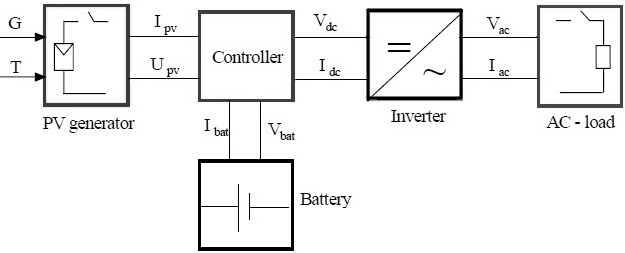
\includegraphics[width=0.4\textwidth]{blockdiagramPVS2}
\centering
\caption{Block diagram for a typical stand-alone PV system~\cite{Hansen}.}
\label{fig:blockdiagram} 
\end{figure}
\\

The sizing check will be performed by the proposed tool, and this stage ensures that the system meets the standard project steps related to critical period solar energy method~\cite{Pinho} and adopting MPPT (Maximum Power Point Tracking) charge controller, that is the most common nowadays. 
%
Firstly, we need to correct the energy consumption estimated to the load ($E_{consumption}$), which is carried out by~\eqref{eq:Ecorrected}, where the efficiency of batteries ($\eta_{b}$), controller ($\eta_{c}$), and the inverter ($\eta_{i}$) are considered~\cite{Pinho} as follows
\begin{equation}
\label{eq:Ecorrected}
\scriptstyle E_{corrected} = \dfrac{\scriptstyle E_{consumption}}{ \scriptstyle \eta_{b} \eta_{c} \eta_{i} }.
\end{equation}

We also need to estimate the energy that can be produced for each panel, called $E_{p}$, in Wh, as defined by~\eqref{eq:Ep}.

\begin{equation}
\label{eq:Ep}
\scriptstyle E_{p} = \scriptstyle Solar\_Irradiance \times Panel\_Area \times \eta_{p} \times 1000,
\end{equation}

\noindent where the solar irradiance is expressed in terms of $kWh/m^{2}$ and depends on the site where the PV systems will be deployed; the PV panel area is given in $m^{2}$ and corresponds to the size of one PV panel, and $\eta_{p}$ represents the PV panel efficiency.
%
The total minimum number of needed solar panels ($N_{TPmin}$) is computed by~\eqref{eq:NTPmin} as
\begin{equation}
\label{eq:NTPmin}
\scriptstyle N_{TPmin} = \dfrac{\scriptstyle E_{corrected}}{\scriptstyle E_{p}}.
\end{equation}

Particularly, the total number of panels in series ($N_{PSmin}$) and parallel ($N_{PPmin}$) are given by~\eqref{eq:NPSmin} and \eqref{eq:NPPmin}, respectively.  
%
\begin{equation}
\label{eq:NPSmin}
\dfrac{\scriptstyle V_{mppt,min}}{\scriptstyle V_{maxPower,TempMax}} \scriptstyle \leq \scriptstyle N_{PSmin} \leq \dfrac{\scriptstyle V_{mppt,max}}{\scriptstyle V_{maxPower,TempMin}}
\end{equation}

\begin{equation}
\label{eq:NPPmin}
\scriptstyle N_{PPmin} = \dfrac{\scriptstyle P_{total}}{\scriptstyle Number\,Panels\,Series \scriptstyle \times \scriptstyle P_{max,ref}},
\end{equation}

\noindent where $V_{mppt,max}$ is the maximum operation voltage and $V_{mppt,min}$ is the minimum operation voltage of the charge controller; $V_{maxPower,TempMax}$ and $V_{maxPower,TempMin}$ are the maximum power voltage from the PV module considering the maximum and minimum operational temperature, respectively; $P_{total}$ is the total power demanded from the PV system and $P_{max,ref}$ is the power supplied from one PV panel in $Watts$.
%, $ V_{system} $ is the DC voltage of the bus, normally $12$, $24$ or $48$ V.
%
Regarding the batteries, we must first define the total capacity of the battery bank, as described by~\eqref{eq:Cbank} as
\begin{equation}
\label{eq:Cbank}
\scriptstyle C_{bank} \scriptstyle = \dfrac{\scriptstyle E_{corrected} \scriptstyle \times \scriptstyle autonomy}{\scriptstyle V_{system} \scriptstyle \times \scriptstyle DOD},
\end{equation}
%
\noindent where the variable $autonomy$ is a design definition; % and normally has a value ranging from $6$ to $48$h; 
$ V_{system} $ is the DC voltage of the bus, and $ DOD $ is the battery deep of discharge (considered of maximum of 25\% at this paper).
%
Secondly, the total (minimum) number of batteries is computed, as described by \eqref{eq:Nbtotal}. 
\begin{equation}
\label{eq:Nbtotal}
\scriptstyle N_{B}total = \scriptstyle N_{BS}min \scriptstyle \times \scriptstyle N_{BP}min = \dfrac{\scriptstyle V_{system}}{\scriptstyle V_{bat}} \scriptstyle \times \dfrac{\scriptstyle C_{bank}}{\scriptstyle 1 \,Battery \, Capacity}.
\end{equation}

Related to the charge controller, initially it must meet the voltage requirement of the PV system, as described by ~\eqref{eq:vcvsystem} to the charge controller voltage: 
\begin{equation}
\label{eq:vcvsystem}
\scriptstyle V_{c} = \scriptstyle V_{system}.
\end{equation}

Following, the short circuit reference information from the manufacturer's solar panel must be corrected to the cell temperature, as described by \eqref{eq:iscamb}:
%
\begin{equation}
\label{eq:iscamb}
\scriptstyle I_{sc,amb} = \dfrac{\scriptstyle G}{\scriptstyle G_{ref}} \left[ \scriptstyle I_{sc,ref} + \scriptstyle \mu_{I} \scriptstyle \times \scriptstyle (T-25) \right]. 
\end{equation}

The controller must meet the maximum current from the PV array given by \eqref{eq:icmin} and \eqref{eq:icicmin}.
\begin{equation}
\label{eq:icmin}
\scriptstyle I_{c,min} = \scriptstyle I_{sc,amb} \times \scriptstyle N_{PP}.
\end{equation}

\begin{equation}
\label{eq:icicmin}
\scriptstyle I_{c} \geq \scriptstyle I_{c,min}.
\end{equation}

The sizing project check of the inverter is carried out by means of three equations. Equation~\eqref{eq:vindc} ensures that the input voltage of the controller meets the system voltage. Equation~\eqref{eq:voutac} ensures that the output voltage of the controller meets the AC voltage of the load. Finally, \eqref{eq:invcheck} ensures that the controller can support the total demand of the load ($Demand$) and the surge power ($P_{surge}$). Where $V_{in}DC$ is the nominal input voltage and $V_{out}AC$ is the nominal output voltage of the inverter; $MAX_{AC,ref}$ is the peak power that the inverter can support.
%
\begin{equation}
\label{eq:vindc} 
\scriptstyle V_{in}DC = \scriptstyle V_{system}.
\end{equation}
%
\begin{equation}
\label{eq:voutac} 
\scriptstyle V_{out}AC = \scriptstyle V_{AC}.
\end{equation}
%
\begin{equation}
\label{eq:invcheck} 
\left[ (\scriptstyle Demand \leq \scriptstyle P_{AC,ref}) \, \scriptstyle and \, \scriptstyle (P_{surge} \leq MAX_{AC,ref}) \right].
\end{equation}
% -------------------------------------------------------
\subsection{Optimum sizing of PV systems}
% -------------------------------------------------------
To select an optimum combination of compontntes from a PV system in order to meet sizing constraints, we need to evaluate \textit{power reliability} and perform \textit{system cost} analysis for the recommended system. An ideal combination for any PV system is made by the best compromise between those two objectives (power reliability and system cost)~\cite{Alsadi2018}. 

Regarding power reliability, this work will rely on the critical period solar energy method~\cite{Pinho} as described in section~\ref{sec:sizing}.
%the usual is to use loss of load probability (LOLP) or loss of power supply probability (LPSP). Based on the fact that here we are neither considering site characteristics nor the load changes over time, the reliability analysis will be developed only by the critical period method of PV sizing \textcolor{red}{What does it mean? Remember that we have software engineering audience}. 

However, considering the system cost analysis, we usually find related studies done with Net Present Cost (NPC), Levelized Cost of Energy (LCOE) or Life Cycle Cost (LCC). Here, based on the fact that the local of deployment is not specified, our study uses an adapted LCC analysis, where only the deployment cost is considered about the model, i.e., without the operational and maintenance costs~\cite{Alsadi2018}.
%------------------------------------------------------
\section{APPLYING AUTOMATED VERIFICATION TO OPTIMAL SIZING OF STAND-ALONE PV SYSTEMS}
%Applying Automated Verification to Optimal Sizing of Stand-alone Solar PV Systems}
%------------------------------------------------------

Algorithm~\ref{alg:verification-algorithm} describes the pseudocode used to optimize stand-alone PV systems using automated verification. 
%
 \begin{algorithm}
 \caption{Optimization algorithm}
 \begin{algorithmic}[1]
 \begin{scriptsize}
 
 \renewcommand{\algorithmicrequire}{\textbf{Input:}}
 \renewcommand{\algorithmicensure}{\textbf{Output:}}
  \STATE $initialize \, variables$ \\
  \STATE $declare \, list \, of \, PV \, panels \, data \, and \, cost $ \\
  \STATE $declare \, list \, of \, controllers \, data \, and \, cost $ \\
  \STATE $declare \, list \, of \, batteries \, data \,  and \, cost $ \\
  \STATE $declare \, list \, of \, inverters \, data \,  and \, cost $ \\
  \STATE $declare \, the \, maximum \, cost \, possible \, MaxCost $  \\
  \STATE $declare \, power \, demand, \, power \, peak, \, energy \, consumption $ \\
  \STATE $declare \, battery\,  autonomy, deep \, of \, discharge, AC \, voltage$ \\
  \FOR {$HintCost=0$ to $MaxCost$}
 	\STATE $declare \, non-det \, variable \, to \, select \, Panel \, from \, list$ \\
 	\STATE $declare \, non-det \, variable \, to \, select \, Controller \, from \, list $ \\
 	\STATE $declare \, non-det \, variable \, to \, select \, Battery \, from \, list $ \\
 	\STATE $declare \, non-det \, variable \, to \, select \, Inverter \, from \, list $ \\ 	
 	\STATE $calculate \, E_{corrected}, \, E_{p} $ \\
	\STATE $calculate \, N_{TPmin}, \, N_{PSmin}, N_{PPmin} $ \\
 	\STATE $calculate \, C_{bank}$ \\
	\STATE $calculate \, N_{BS}min, \, N_{BP}min, \, N_{B}total$ \\
	\STATE $requeriment \, enforced \, by \, \textbf{assume}(V_{c})$ \\
 	\STATE $calculate \, I_{sc,amb}$ \\
 	\STATE $calculate \, I_{c,min}$ \\
 	\STATE $requeriment \, enforced \, by \, \textbf{assume}(I_{c})$ \\
	\STATE $requeriment \, enforced \, by \, \textbf{assume}(V_{in}DC)$ \\
	\STATE $requeriment \, enforced \, by \, \textbf{assume}(V_{out}AC)$ \\
	\STATE $requeriment \, enforced \, by \, \textbf{assume}(Demand)$ \\
	\STATE $requeriment \, enforced \, by \, \textbf{assume}(P_{surge})$ \\
	\STATE $non-det \, variables \, hold \, feasible \, equipment \, and \ cost $ \\
	\STATE $F_{obj} \leftarrow  N_{TP}*Panel_{Cost} \, + \, N_{TB}*Battery_{Cost} \, + Controller_{Cost} \, + \, Inverter_{Cost}$ \\
	\STATE $Violation \, check \, with \, \textbf{assert}(F_{obj} > HintCost)$ \\
  \ENDFOR
 \RETURN $(\,)$ 
  \end{scriptsize}
 \end{algorithmic} 
 \label{alg:verification-algorithm}
 \end{algorithm}
 
Our algorithm starts with the input of manufacturers data and prices of PV panels, batteries, charge controllers and inverters (Lines 2 to 5). After that, we define user requirements, i.e., house requirements and design definitions, from Lines 6 to 8. The \textit{for}-loop started at Line 9 controls the lowest cost to the PV solution. In particular, it starts with cost $0$ and stops only when the algorithm finds a feasible solution in which the cost breaks the assertion stated in Line 28; if that happens, then our algorithm has found an optimum solution, stating that the automatic verification reached a \textit{SAT} (satisfiable) condition. The algorithm uses non-deterministic variables to choose one specific data from a list of PV panels, controllers, batteries and inverters (Lines 10 to 13). That procedure ensures that the automated verification checks all possibilities of items from each equipment, and combine them to assemble a feasible PV solution, which meets the user requirements.

Next, we use Eq.~(\ref{eq:Ecorrected}), Eq.~(\ref{eq:Ep}), Eq.~(\ref{eq:NTPmin}), Eq.~(\ref{eq:NPSmin}), Eq.~(\ref{eq:NPPmin}), Eq.~(\ref{eq:Cbank}), Eq.~(\ref{eq:Nbtotal}), Eq.~(\ref{eq:iscamb}), and Eq.~(\ref{eq:icmin}) to calculate the sizing variables (Lines 14 to 20). The directive \textit{assume} (from Line 21 to 25) ensures the compatibility of the chosen items from the list of equipment: the automatic verification uses only the item (among all the possible ones) that satisfies the statements from Line 14 to 20 in addition to the Line 18. Therefore, our algorithm reaches Line 27 with one feasible solution, and the cost of that solution is calculated in $F_{obj}$.

If our algorithm does not find a feasible solution among the item of equipment that were inputted to the code, then the result is an \textit{UNSAT}, i.e., the program finishes and does not find a solution. It indicates that was not possible to combine the itens of each equipment and create a feasible solution.

\textcolor{red}{The main challenge for the verification part is to found a feasible solution (technically speaking, regarding the constraints and user requirements) that is the best financial solution at the same time (lowest cost of deployment) from a list of equipment and components that is inputted to the tool}.
%---------------------------------------------------------------------------
\section{RESULTS AND DISCUSSION}
%---------------------------------------------------------------------------
We have performed two case studies to evaluate the proposed approach of optimization as described in Table~\ref{tab1}. Furthermore, three start-of-art verification tools, as described in Section~\ref{sec:AutomatedVerification}: CBMC\footnote{Command-line: \$ cbmc -\phantom{}-unwind 100 filename.c -\phantom{}-trace}, ESBMC\footnote{Command-line: \$ esbmc filename.c -\phantom{}-no-bounds-check -\phantom{}-no-pointer-check -\phantom{}-unwind 100 -\phantom{}-boolector}, %UAutomizer\footnote{Command-line: \$ ./Ultimate -tc config/AutomizerReach.xml -s config/svcomp-Reach-32bit-Automizer\_Default.epf -i filename.c -\phantom{}-traceabstraction.limit.analysis.time 900 -\phantom{}-traceabstraction.stop.after.first.violation.was.found false -\phantom{}-cacsl2boogietranslator.overapproximate.operations.on.floating.types false -\phantom{}- cacsl2boogietranslator.assume.nondeterminstic.values.are.in.range false -\phantom{}-rcfgbuilder.add.additional.assume.for.each.assert true -\phantom{}-rcfgbuilder.simplify.code.blocks true -\phantom{}-rcfgbuilder.size.of.a.code.block LoopFreeBlock}, 
and CPAchecker\footnote{Command-line: \$ scripts/cpa.sh -heap 64000m -config config/bmc-incremental.properties -spec config/specification/sv-comp-reachability.spc filename.c}, were used to compare the approach effectiveness and efficiency. The case studies are related to a stand-alone PV system with the specifications shown in Table~\ref{tab1}.

All experiments were conducted on an otherwise idle Intel Xeon CPU E5-4617 (8-cores) with 2.90 GHz and 64 GB of RAM, running Ubuntu 16.04 LTS 64-bits. The experiments were performed with a predefined timeout of 240 minutes.

%used with the SMT incremental mode\footnote{Command-line: \$ esbmc filename.c -\phantom{}-no-bounds-check -\phantom{}-no-pointer-check -\phantom{}-unwind 100 -\phantom{}-smt-during-symex -\phantom{}-smt-symex-guard -\phantom{}-z3} enabled with the goal of reducing memory usage; we have also used the SMT solver Z3 version 4.7.1~\cite{DeMoura}.
\begin{table}
\caption{Case studies and Results: optimization of PV systems.}\label{tab1}
\begin{scriptsize}
\begin{tabular}{|c|c|c|}
\hline
\hline
 & Case 1 & Case 2\\
\hline
\hline
Tool & \makecell{Demand = 501W \\ Peak = 501W \\ Energy=3900Wh/day \\ Battery autonomy=48h} & \makecell{Demand = 915W \\ Peak = 980W \\ Energy=4880Wh/day \\ Battery autonomy=6h}\\
\hline
\makecell{CBMC 5.11 \\(MiniSat 2.2.1)} & \makecell{UNKNOWN \\(Out of Memory)} & \makecell{UNKNOWN \\(Out of Memory)}\\
\hline
\makecell{ESBMC 6.0.0 \\(Boolector 3.0.1)} & \makecell{UNKNOWN \\(Timeout)} & \makecell{UNKNOWN \\(Timeout)} \\
\hline
%UAutomizer 0.1.24 (Z3 4.8.3) & UNKNOWN & UNKNOWN \\
%\hline
\makecell{CPAchecker 1.8 \\(MathSAT 5.5.3)} & \makecell{SAT (66.18 min) \\ Property violation line 195: \\NTP= 4 $\times$ 320W model (2S-2P)\\NBT= 4 $\times$ 105Ah model (2S-2P)\\ Controller 15A/100V\\Inverter 700VA, 48V \\ Total Cost: US\$ 2,643.00} & \makecell {SAT (35.41 min) \\ Property violation line 195:  \\NTP= 3 $\times$ 320W model (3S)\\NBT= 2 $\times$ 105Ah model (2S)\\ Controller 35A/145V \\ Inverter 1,200VA, 48V \\ Total Cost: US\$ 2,125.00}\\
\hline
\hline
\end{tabular}
\end{scriptsize}
\end{table}

More experimentation will be performed with a larger number of case studies and to compare the result with some off-the-shelf software that focus on sizing and optimization (validation of the result). Besides, it will be inputted a larger number of components (panels, batteries, contollers and inverters) to the database (that is limited to 12 items right now). That will bring more complexity to the tool, however will ensure an even better optimization.
% argument is your BibTeX string definitions and bibliography database(s)
\bibliography{trindadeThesis}{}

\vspace{12pt}

\end{document}
